\section{XMD - XMV integration}

\subsection{QML}

The xMAS model designer was created in QML. QML is a declarative language
that promotes quick design of user interfaces. In fact, QML is a complete javascript language
with some extra features for Qt, like support for {\sc QString}. 
The language uses a declarative, JSON-like syntax that allows developers to describe 
visual components and their interactions in a readable and compact notation. Being 
a javascript language, the programmer can use all expressions available
in javascript while enjoying Qt enhancements. 
Additionally, QML provides a C++ API for back-end C++ libraries that connects both environments
transparantly.

\subsection{User interface}

The user interface consists of multiple qml files in two folders.
The folder {\tt uicontrols} contains controls like the toolbar, 
console and dialogs. These QML files make up the user interface. 
The folder {\tt xobjects} contains QML files to draw the 
xMAS components on the designer canvas. 

Finally, the file {\tt mainWindow.qml} represents the root of the interface definition.

\paragraph{Separation of code}
The QML language contains both procedural code (javascript) and declarative code (JSON).
Several {\tt .js} files contain the procedural logic. The {\tt .qml} files contain
the declarative code plus a few snippets of javascript logic limited to one or two lines. 
The division of declarative and procedural code promotes clean, uncluttered code. 
The ability to include {\tt .js} files into a qml file promotes reuse of code.

\subsection{C++ integration}
QML objects can interact with each other and with their C++ counterparts 
either directly by accessing their property values or through the signal/slot mechanism. 
Interaction between QML and C++ classes is more complicated than the QML internal
interaction. Especially the timing of coordination could result in surprises for
the unsuspecting QML/C++ programmer who is well served reading the official QML documentation
in case of problems. 

The application uses two methods provided by QML to integrate QML and C++ objects.

\subsubsection{QML Context property}
Each QML application operates in a certain QML context. The QML context stores
properties that are available throughout all QML code. Registration of C++ classes 
with the Qt metasystem exposes the C++ classes to the QML world.
Registration adds a C++ object instance to the QML context using a property value.
XMD uses context properties to provide access to three C++ classes:

\begin{itemize}
 \item \textbf{datacontrol} (of class DataControl) to provide access to the
 underlying xMAS data model to both QML and the other C++ classes
 \item \textbf{plugincontrol} (of class PluginControl) to provide access to
 the plugins that manage starting and stopping of verification tools. Only Qml
 uses the plugin control program.
 \item \textbf{util} (of class Util) to provide utility functions for C++.
\end{itemize}

\begin{figure}
    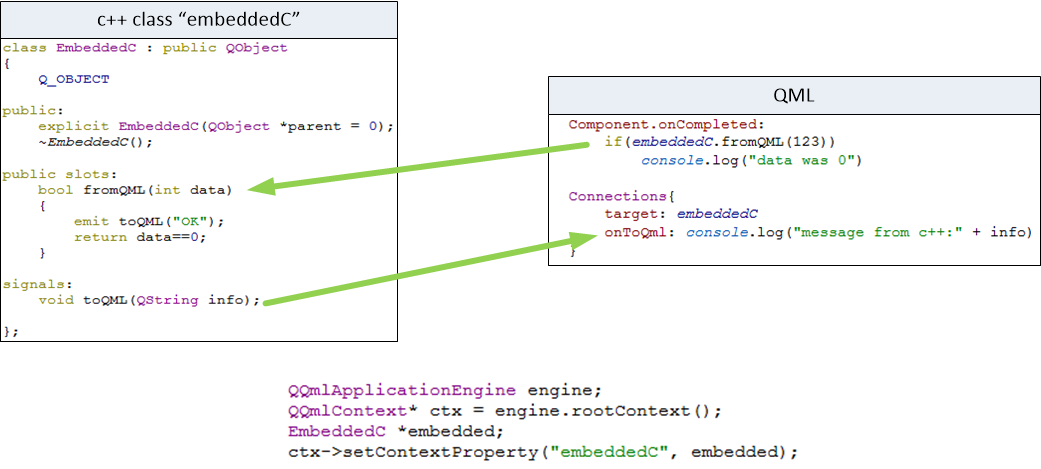
\includegraphics[width=\textwidth]{qml3}
    \caption{Registering a QML context property}
\end{figure}

\paragraph{QML Documentation}
More information on context properties is available at:
\url{http://doc.qt.io/qt-5/qtqml-cppintegration-contextproperties.html}


\subsubsection{Embedding C++ classes in QML}

One can extend QML applications with C++ code by registering C++ classes
with the QML type system. Any C++ class that derives from QObject connect to QML this way.
Registering the class with QML not only allows access to the properties,
methods and signals of an object. Additionally, QML code can directly instantiate
new objects of the registered classes (see figure \ref{fig:register-qml}).

\begin{figure}
    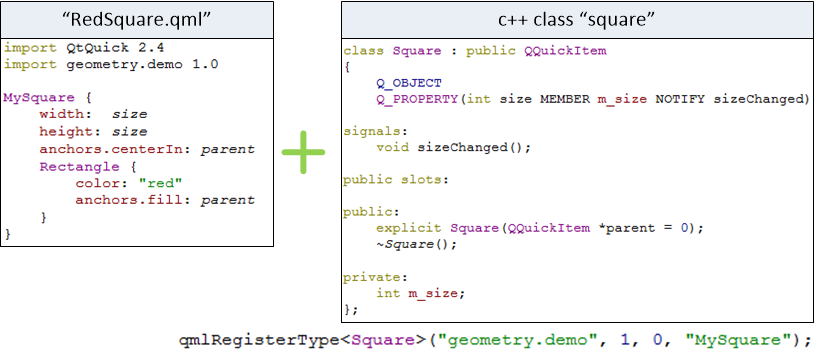
\includegraphics[width=\textwidth]{qml1}
    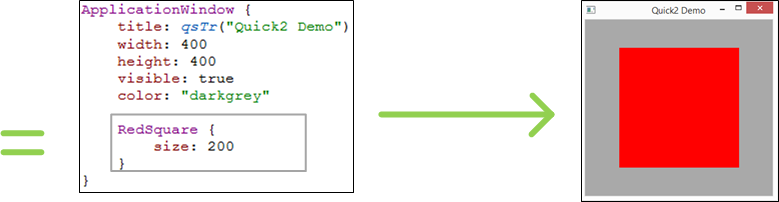
\includegraphics[width=\textwidth]{qml2}
    \caption{Exposing a C++ class to QML}
    \label{fig:register-qml}
\end{figure}

\paragraph{Usage}XMD registers four C++ classes to the QML type system. These classes
are \textsc{Channel}, \textsc{XPort}\footnote{This class has been named XPort to
avoid confusion with the Port class defined in the xMAS data model. Any confusion
in names can lead the QML/C++ API astray and could lead to difficult to find errors.}, 
\textsc{Network} and \textsc{Component}. 
The definitions of each of the four classes is split into three files. 
The {\tt .h} and {\tt .cpp} files contain normal C++ header and source files of the 
classes. Furthermore, each class has a QML file, e.g. XChannel.qml, which contains
additional QML code (figure \ref{fig:qml-cpp-classes}). All three files belong to
the same class. Even though the class names are sometimes different (e.g. Channel vs.
XChannel), the QML type system binds the C++ code and the QML code together to form a
single class definition. Registration of types is done by a call to qmlRegisterType,
figure \ref{fig:register-qml} shows an example.

\paragraph{QML Documentation}
More information is available at:
\url{http://doc.qt.io/qt-5/qtqml-tutorials-extending-qml-example.html}

\begin{figure}
    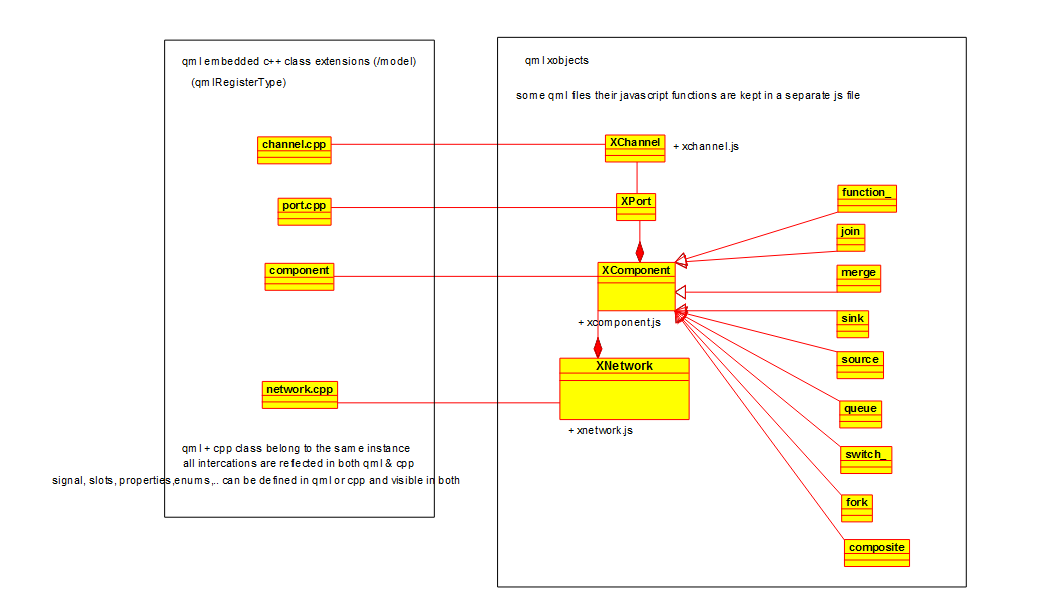
\includegraphics[width=\textwidth]{qml-cpp-extension}
    \caption{Qml/ C++ integration by extending the QML type system}
    \label{fig:qml-cpp-classes}
\end{figure}

\subsubsection{Interaction xmd / datamodel classes}

See figure~\ref{fig:xmd-xmv-integration} for an overview of the 
\textsc{Xmd-Xmv} integration.

\begin{figure}
    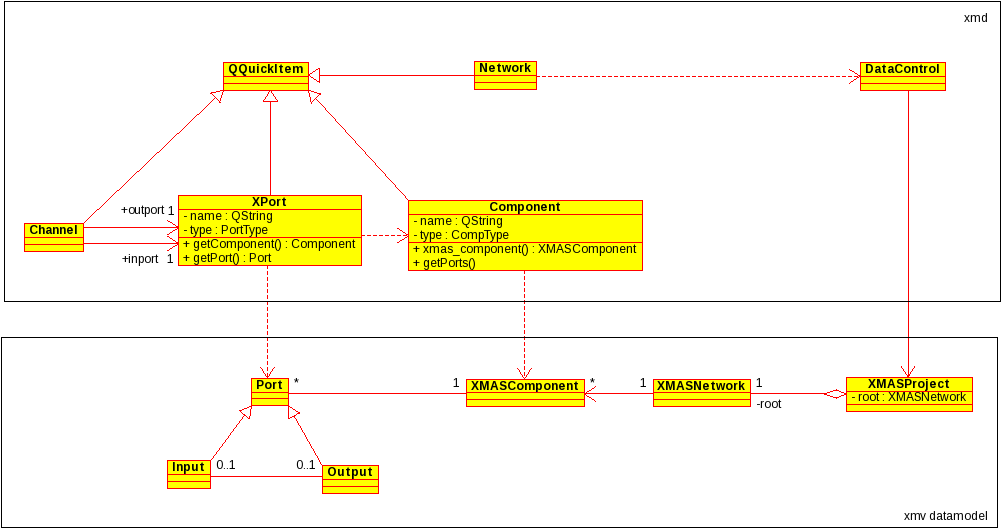
\includegraphics[width=\textwidth]{xmd-xmv-integration}
    \caption{Integration of xmd and xmv datamodel}
    \label{fig:xmd-xmv-integration}
\end{figure}

%\newpage
\subsubsection{Architecture}

See figure~\ref{fig:global-system-architecture} for an overview
of the system architecture.

\begin{figure}[ht]
    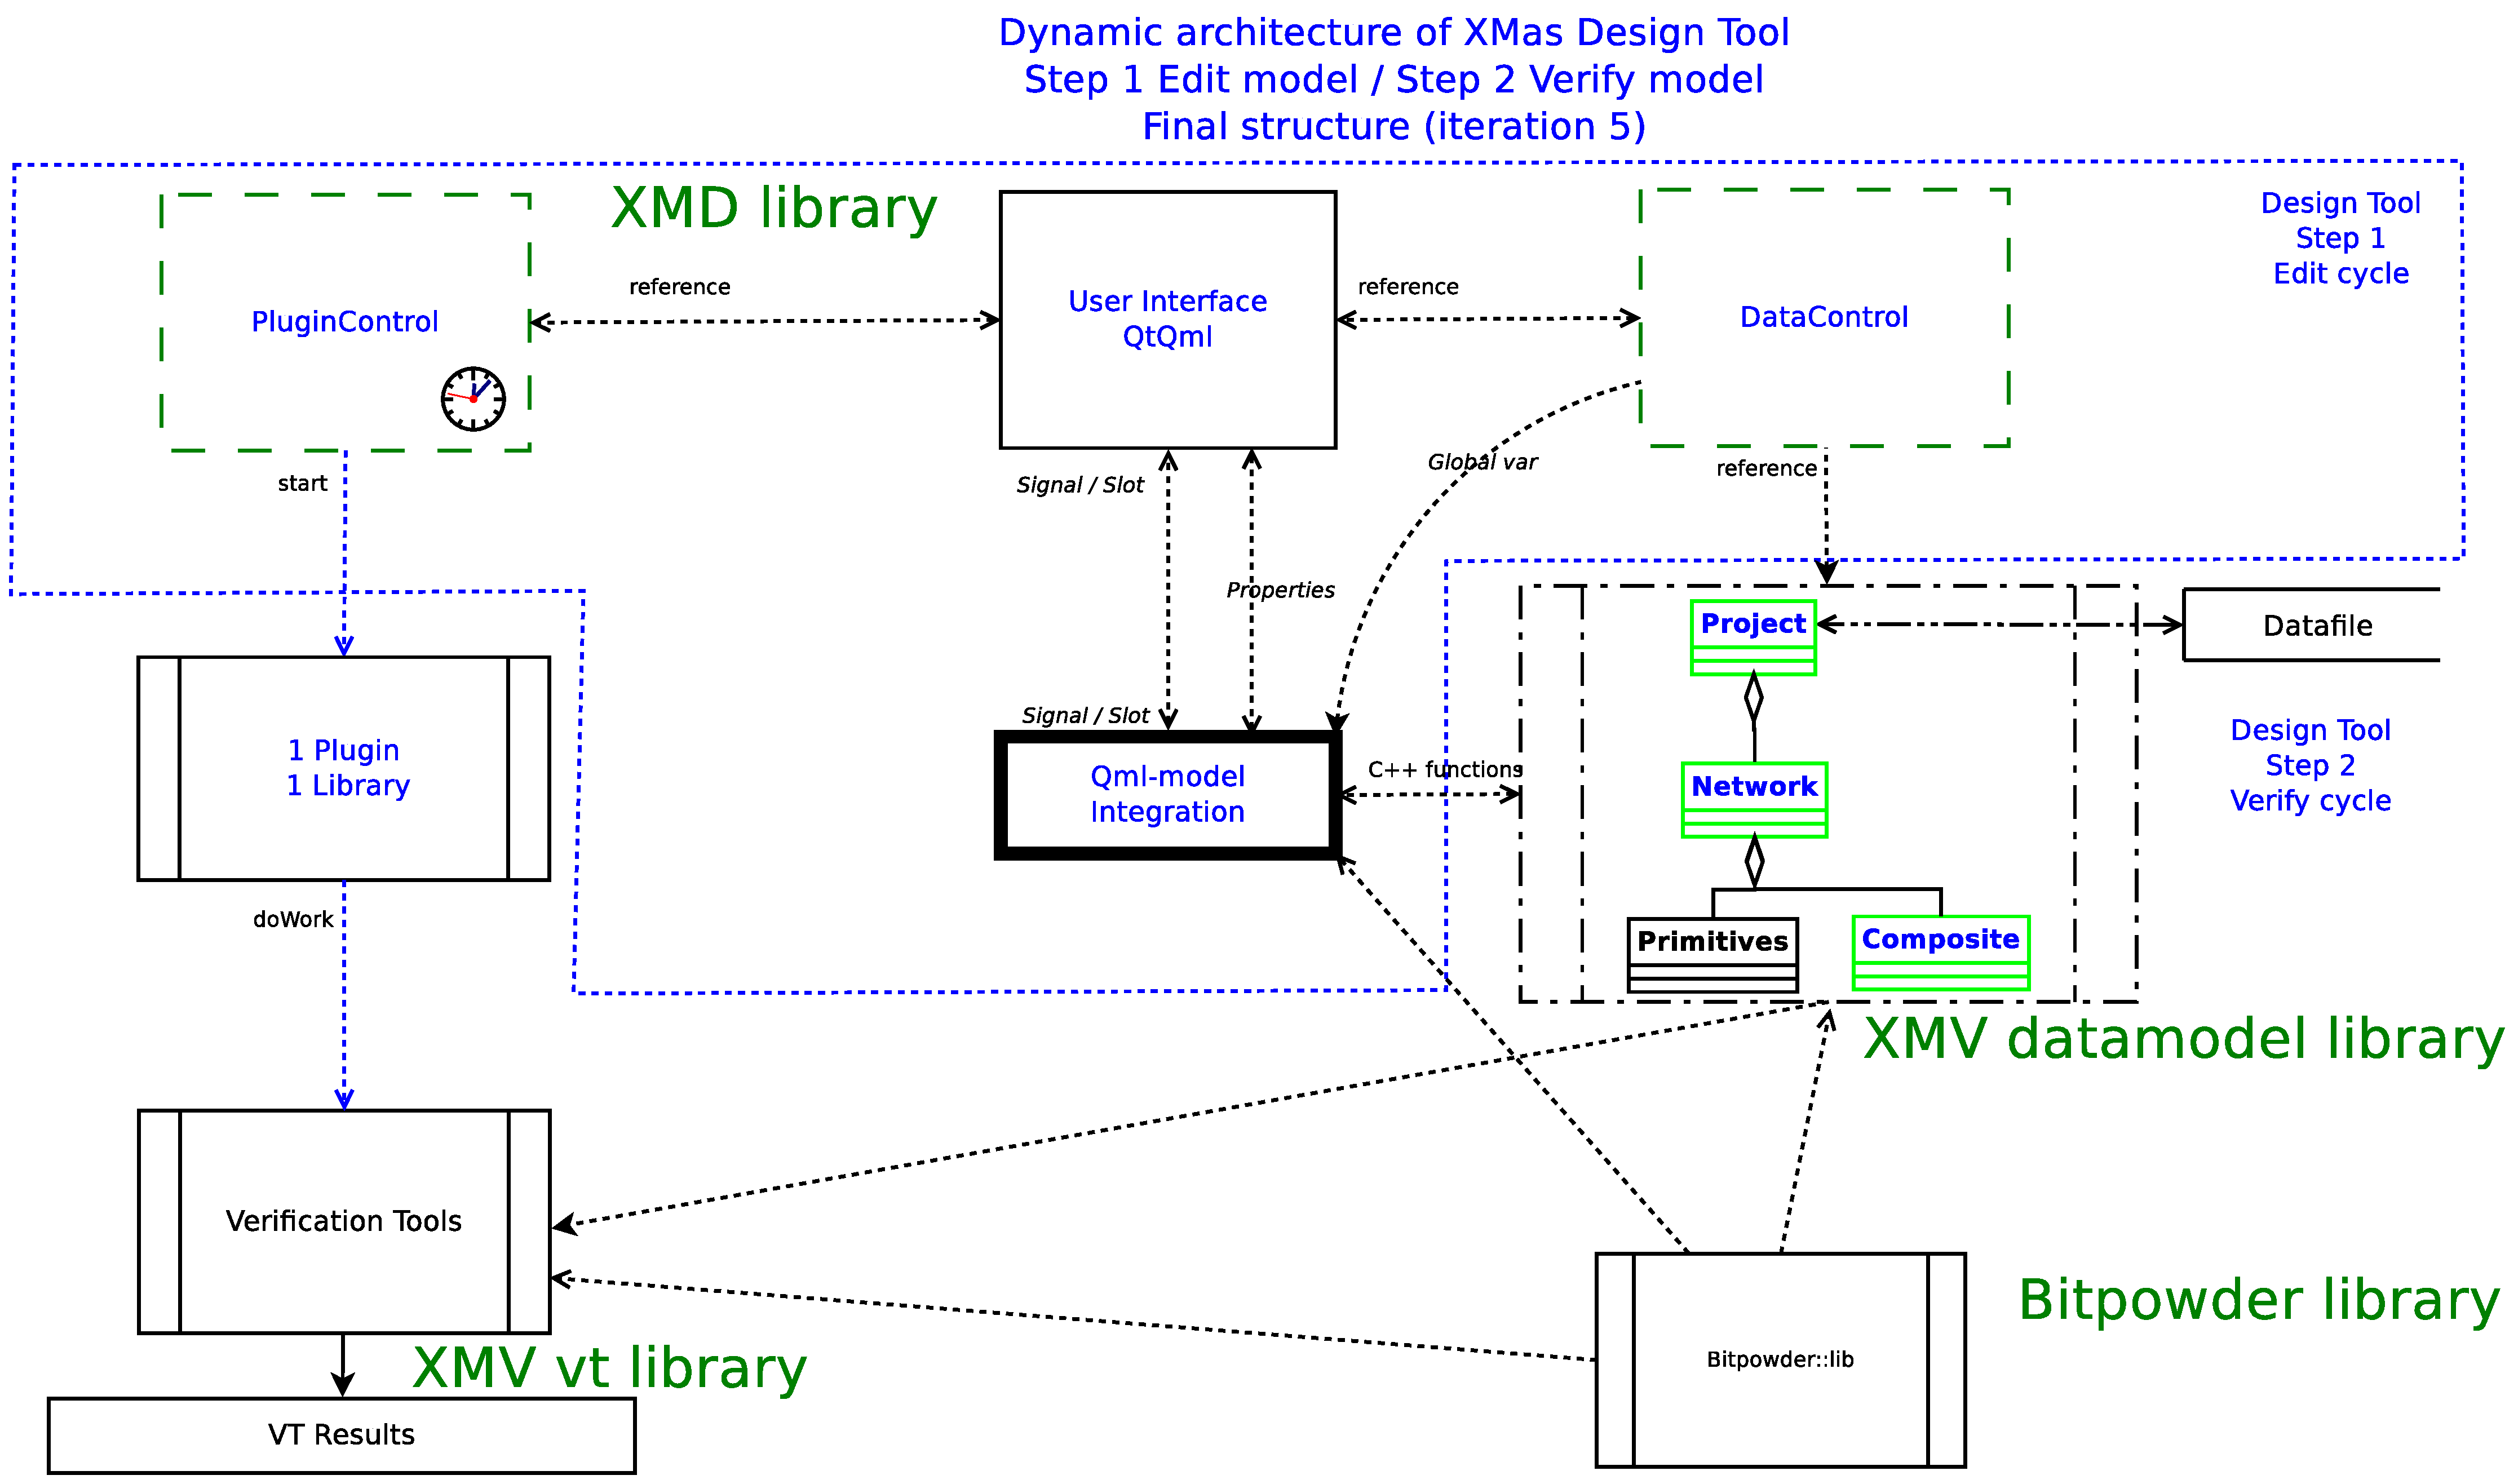
\includegraphics[width=\textwidth]{1c-architecture-dynamic-2}
    \caption{Global system architecture}
    \label{fig:global-system-architecture}
\end{figure}
